\subsection{Hardware}\label{subsection:A}
This section contains all hardware used in this capstone project.
    \subsubsection{Drone Kit}\label{subsection:A1}
    \begin{itemize}
        \item QWinOut Q705 6-Aixs RC Drone (Archive)
        \item QWinOut J630 4-Aixs RC Drone
    \end{itemize}

    \begin{figure}[H]
        \centerline{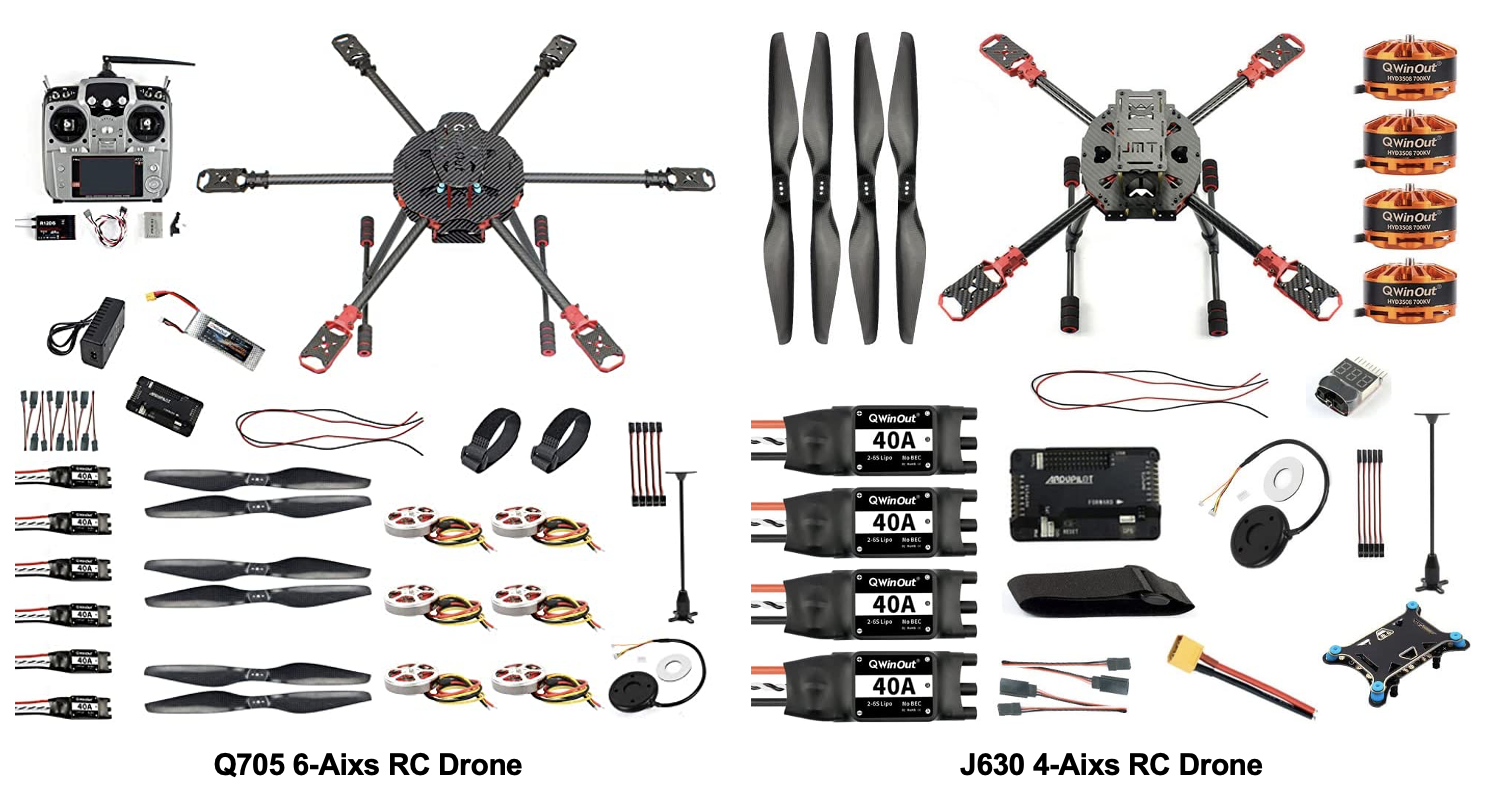
\includegraphics[width=0.5\textwidth]{Figures/Methods/Drone_Kits.png}}
        \caption{(left) 6-Axis RC Drone / (right) 4-Axis RC Drone.}
        \label{fig2a1}
    \end{figure}
    
    There are two types of drones used in the project, as shown in Fig.~\ref{fig2a1}, the larger 6-axis RC drone and the new smaller 4-axis drone purchased in the 2023 spring semester. The larger 6-axis drone is a continuation of the team's work from the previous semester, and the smaller 4-axis drone is a new drone that we assembled in the 2023 spring semester.
    
    \subsubsection{Transistor \& Receiver}\label{subsection:A2}
    \begin{itemize}
        \item SIK Telemetry Radio
        \item Flysky FS-i6   6CH 2.4GHz RC Transmitter
        \item Flysky FS-i6X 10CH 2.4GHz RC Transmitter
        \item iA6B Receiver
        \item iA10B Receiver
    \end{itemize}

    \begin{figure}[H]
        \centerline{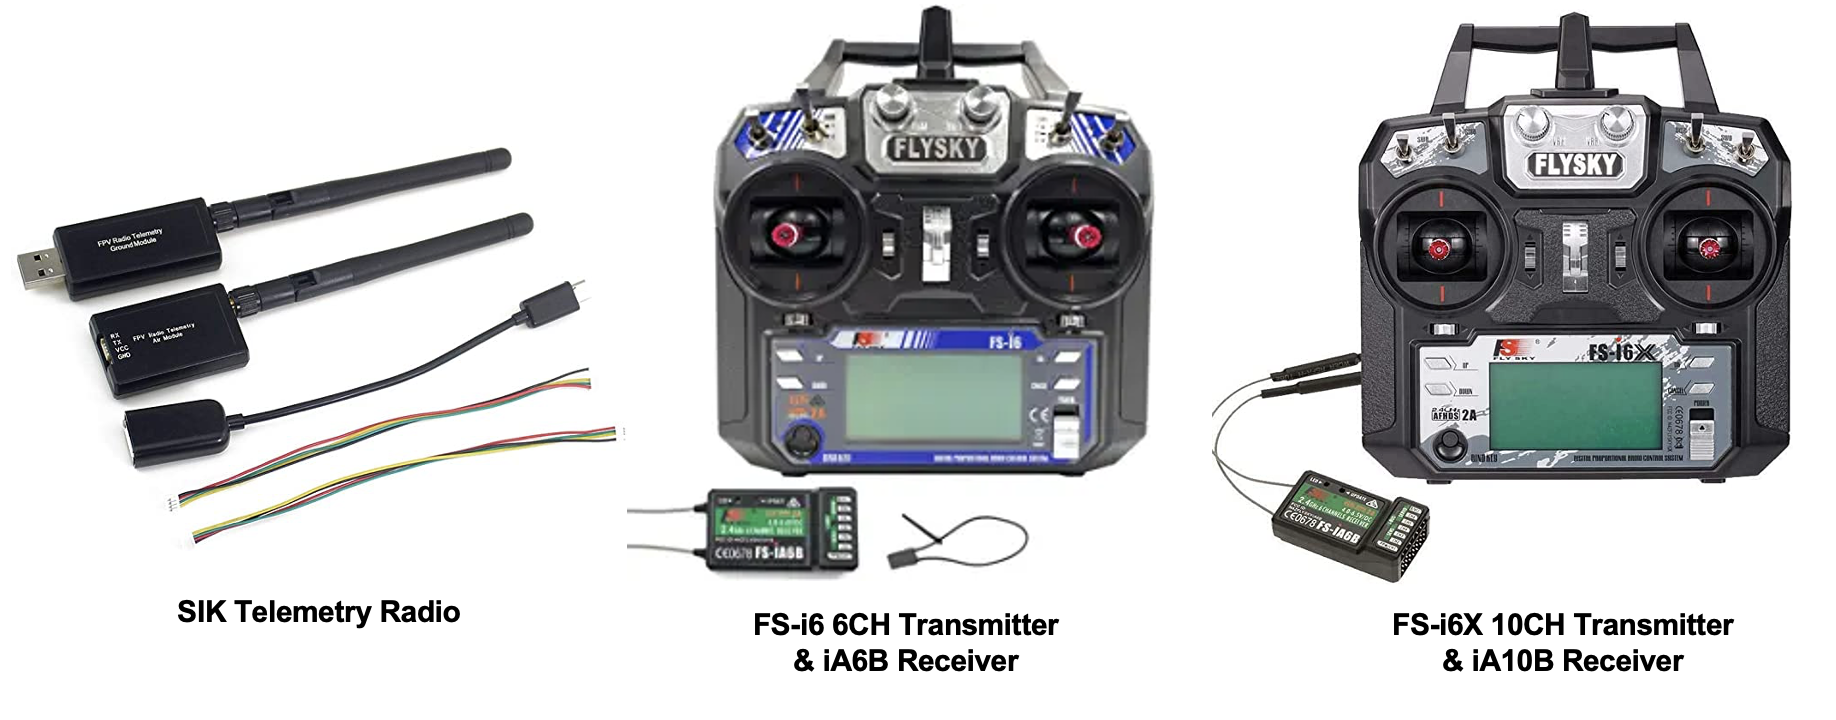
\includegraphics[width=0.5\textwidth]{Figures/Methods/Transistors&Receivers.png}}
        \caption{(left) SIK Telemetry Radio / (middle) FS-i6 6CH Transmitter \& iA6B Receiver / (right) FS-i6X 10CH Transmitter \& iA10B Receiver.}
        \label{fig2a2}
    \end{figure}

    Since we use two types of drones, there are different Transistors \& Receivers for each, as shown in Fig.~\ref{fig2a2}. FS-i6 6CH and iA6B Receiver pairing is for 6-axis drone. FS-i6X 10CH and iA10B Receiver pairing is for 4-axis drone. Then SIK radio just used to communicate between flight controller and Laptop/PC.
    
    \subsubsection{Flight Controller}\label{subsection:A3}
    \begin{itemize}
        \item Cube Black Flight Controller
        \item APM2.8 Flight Controller (Archive)
    \end{itemize}

    \begin{figure}[H]
        \centerline{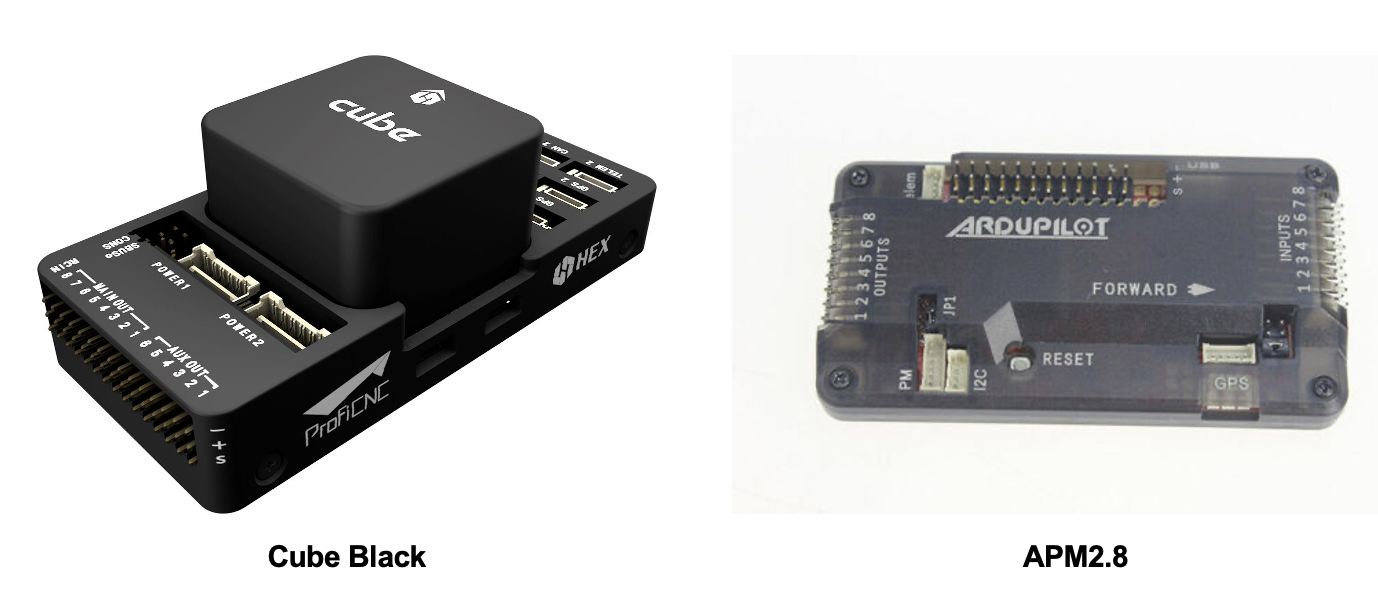
\includegraphics[width=0.5\textwidth]{Figures/Methods/Flight_Controllers.png}}
        \caption{(left) Cube Black / (right) APM2.8.}
        \label{fig2a3}
    \end{figure}

   In the Spring 2023 semester of our project, we employed two flight controller modules, vital for governing the drone's flight and stability. These controllers, processing data from various sensors like accelerometers, gyroscopes, magnetometers, and barometers, ensure optimal altitude, orientation, and movement. Initially, as illustrated in Fig.~\ref{fig2a3}, both the APM2.8 and Cube Black modules were used. However, challenges with calibration and parameter input on the APM2.8 led to its exclusion from the project. Consequently, our focus shifted entirely to utilizing the Cube Black for its superior performance and reliability in flight control operations.
    
    \subsubsection{Embedded System / Controller}\label{subsection:A4}
    \begin{itemize}
        \item Jetson Orin Nano
        \item Raspberry Pi 3B
        \item Raspberry Pi 4B
    \end{itemize}

     \begin{figure}[H]
        \centerline{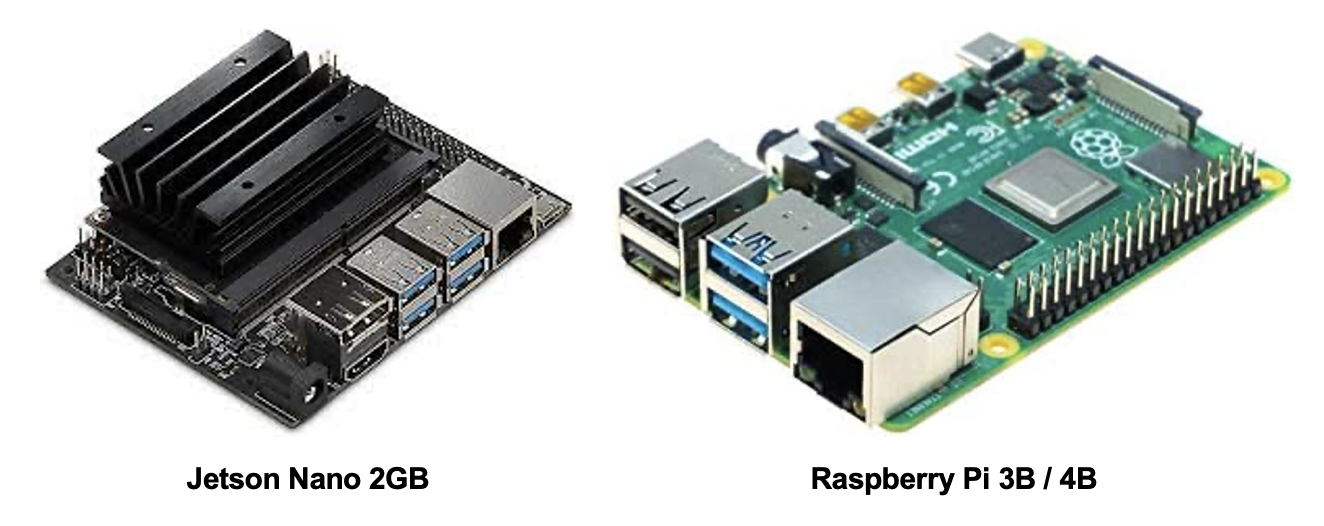
\includegraphics[width=0.5\textwidth]{Figures/Methods/Embedded_Systems.png}}
        \caption{(left) Jetson Orin Nano / (right) Raspberry Pi 3B / 4B.}
        \label{fig2a4}
    \end{figure}

    In the AutoDrone project, our main controller is the embedded system, essential for executing tasks. It captures images from the camera and LiDAR, applying deep learning algorithms for accurate person re-identification and tracking. These algorithms process depth information, guiding the drone's flight controller for precise maneuvering in complex environments.
    
    Our project utilizes two embedded devices: the GPU-equipped Jetson Orin Nano and the smaller Raspberry Pi 3B / 4B, as shown in Fig.~\ref{fig2a4}. We are testing both to assess their compatibility and effectiveness for the project, ensuring optimal performance in real-world scenarios.

    \subsubsection{LiDAR}\label{subsection:A5}
     \begin{figure}[H]
        \centerline{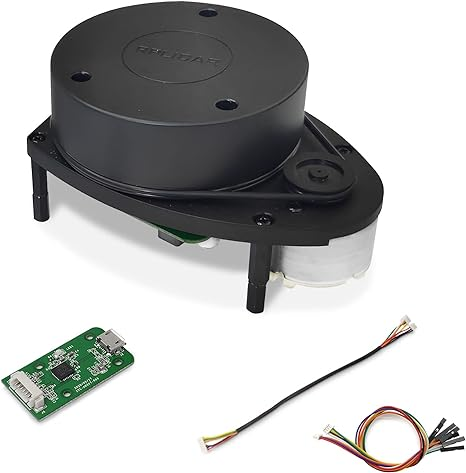
\includegraphics[width=0.2\textwidth]{Figures/Methods/LiDAR.jpg}}
        \caption{LiDAR.}
        \label{fig2a5}
    \end{figure}
    This LiDAR module eas used to detected 2D range around the drone Fig.~\ref{fig2a5}.